\documentclass[%
 reprint,
 amsmath,amssymb,
 aps,
]{revtex4-2}

\usepackage{graphicx}
\usepackage{dcolumn}
\usepackage{bm}
\usepackage{float}
\usepackage{amsmath}

\begin{document}

\title{Determination of Boltzmann's Constant via Brownian Motion and Sedimentation Equilibrium}

\author{Gavin Reider}
\affiliation{Department of Physics, Cornell University}

\date{December 8, 2025}

\begin{abstract}  
I determine Boltzmann’s constant using two complementary measurements of the thermal motion of micron-sized beads suspended in water. First, I analyzed depth-resolved microscope images with particle-tracking software to get bead number density as a function of height. The resulting exponential profile, predicted by the Law of Atmospheres, allowed us to extract $k_B$. Second, I used videos recorded at a fixed depth to track Brownian trajectories, from which I obtained the RMS velocity, diffusion coefficient, and an independent value of $k_B$ using the Einstein–Smoluchowski relation. Both methods produced results consistent with the accepted value, showing how microscopic fluctuations contain fundamental thermodynamic information.  
\end{abstract}  

\maketitle

\section*{Introduction}

Brownian motion is the constant and random movement of tiny particles suspended in a fluid. Robert Brown first described this motion in detail in 1827. While he initially studied pollen grains for biological reasons, he realized that the phenomenon was universal. Even inorganic particles showed the same jittery behavior when placed in a liquid. This observation puzzled scientists throughout the nineteenth century. Conventional hydrodynamic or optical explanations could not clarify the persistent and random nature of the motion. \cite{Brown1866}

A significant theoretical advancement occurred in the early twentieth century through the work of Sutherland, Einstein, and Smoluchowski. Sutherland’s 1905 formulation linked diffusion to the tiny movements of molecules. He showed that the random motion of suspended particles results from countless collisions with the surrounding fluid. This insight led to a statistical understanding of Brownian motion as a direct result of the thermal energy present in all matter. At the same time, scientists developed a statistical-mechanical view of sedimentation equilibrium. When particles are subject to gravity, they create a vertical concentration gradient based on their thermal energy and buoyant mass. This pattern, often called the Law of Atmospheres, reveals another visible sign of the same microscopic fluctuations. \cite{Sutherland1905}

The current experiment uses micron-scale colloidal beads to investigate these two classic phenomena. By imaging the distribution of beads at different focal depths and tracking their changing paths over time, I study how thermal motion influences both their equilibrium position and random behavior. These observations will serve as a basis for later detailed analysis, where the same microscopic fluctuations will help determine a fundamental constant of nature.


\section*{Experimental Methods}

The experiment involved two complementary measurements using a suspension of $1~\mu\text{m}$ diameter polystyrene microspheres in distilled water. All observations were made with a Nikon Diaphot 300 inverted microscope, which had a digital camera mounted on the side port. The sample was prepared by putting a small volume of bead solution between two clean microscope slides to create a thin fluid chamber. After the beads had time to settle, the slide was placed on the microscope stage for imaging.

\subsection*{Sedimentation Imaging}

To measure the vertical distribution of the beads, the microscope's fine-focus drive was used to shift the focal plane in uniform increments of $5~\mu\text{m}$ over a total depth range of $200~\mu\text{m}$. At each step, a still image was captured under consistent lighting and exposure settings. The complete set of images, which included an initial background frame with no sample present, was processed using Trackpy-based particle detection routines. \cite{trackpy} This let us quantify the number of beads visible at each depth, resulting in a depth-dependent concentration profile.

\subsection*{Brownian Motion Recording}

To measure the random motion of beads in the horizontal plane, I recorded short videos at a fixed focal depth near the center of the sample chamber. I chose imaging parameters to ensure good temporal resolution of the bead paths while reducing motion blur. I then tracked individual bead positions across frames using automated particle-tracking algorithms. From these paths, I calculated the instantaneous displacements and velocity distributions for further analysis.

\subsection*{Microscope Setup}

A photograph of the laboratory bench and microscope setup used in this experiment is shown in Fig.~\ref{fig:setup}. This includes the microscope body, light source, camera interface, and sample mounting hardware.

\begin{figure}[H]
    \centering
    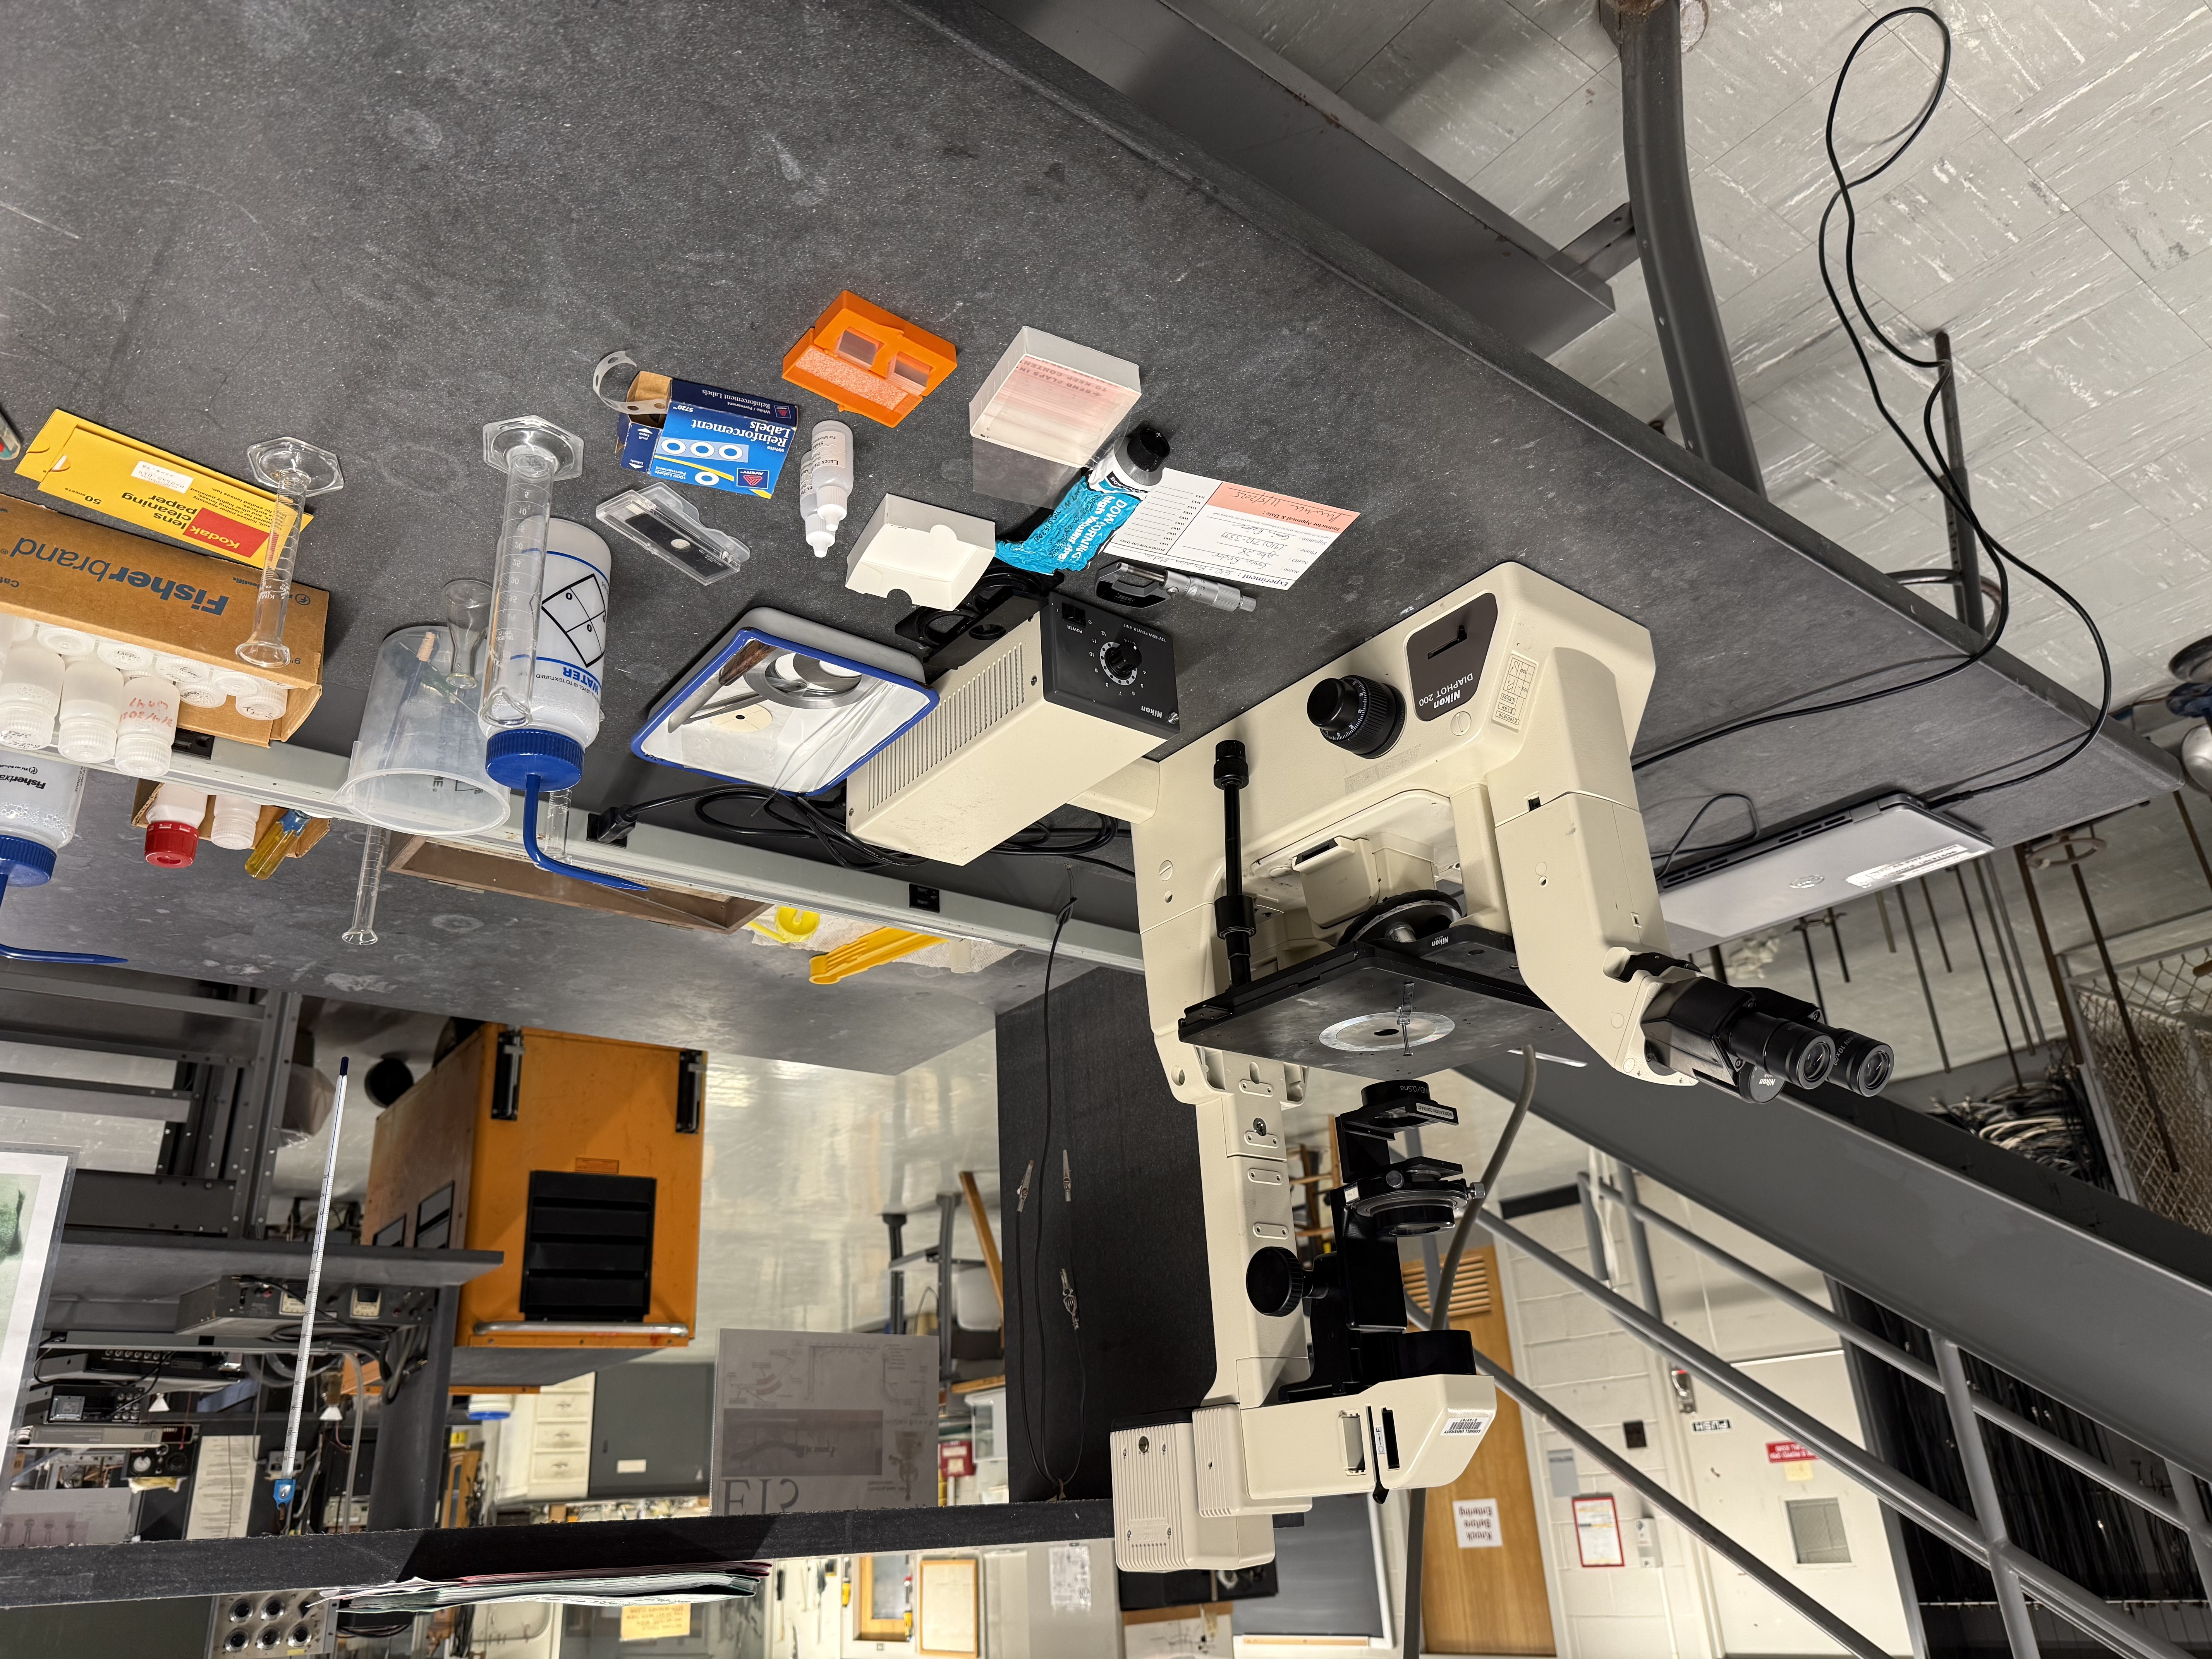
\includegraphics[width=0.45\textwidth, angle=180]{figures/microscope_setup.jpeg}
    \caption{Experimental setup showing the Nikon Diaphot 300 microscope,
    digital camera, and sample positioning hardware.}
    \label{fig:setup}
\end{figure}

\section*{Data and Analysis}

The experiment produced two different datasets: (1) a series of depth-resolved microscope images to measure the equilibrium concentration profile of suspended beads, and (2) video recordings of bead motion to extract the statistics of Brownian trajectories. I analyzed each dataset using Python and the package Trackpy, and custom routines for preprocessing, particle detection, and trajectory reconstruction. \cite{trackpy}

\subsection*{Sedimentation Profile}

To study the vertical distribution of beads, I processed the depth-resolved microscope images and counted the number of particles in each frame. The resulting bead count in relation to depth is shown in Fig.~\ref{fig:sedimentation}. Only the right side of the plot, where the count consistently decreases, corresponds to the sedimentation equilibrium distribution. The left side is affected by particles out of focus and the lower boundary of the sample chamber.

\begin{figure}[t]
    \centering
    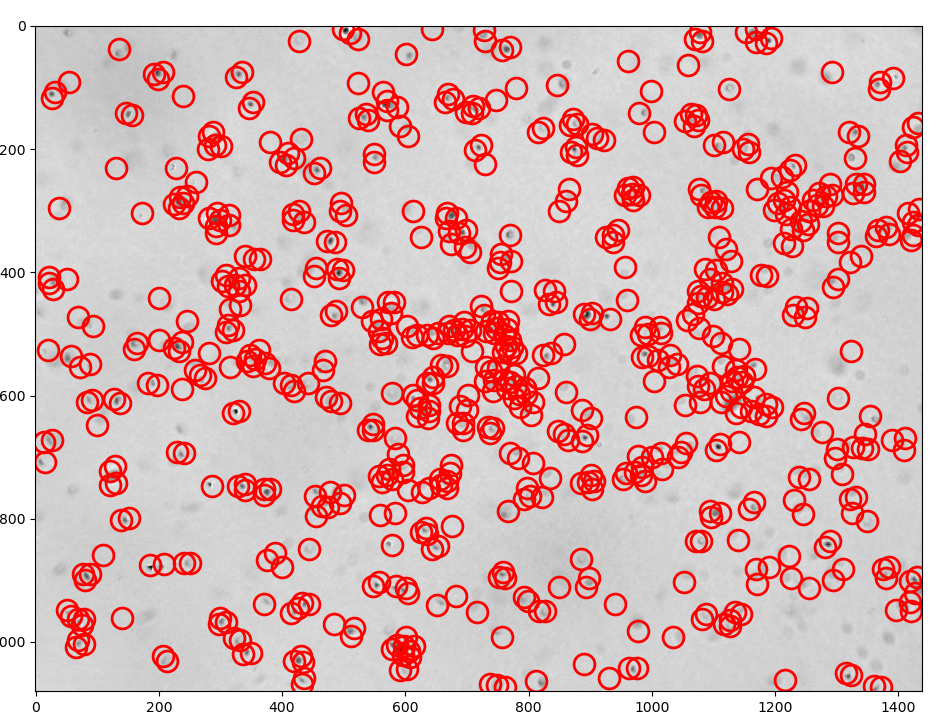
\includegraphics[width=0.48\textwidth]{figures/detected_particles.png}
    \caption{Microscope image of the bead suspension at the optimal depth, with detected particles highlighted by red circles. Particle identification took place using Trackpy after preprocessing. \cite{trackpy} This included background subtraction and bandpass filtering. This visualization shows that the detection algorithm consistently identifies individual beads throughout the field of view.}
    \label{fig:particle_detection}
\end{figure}

\begin{figure}[t]
    \centering
    
\includegraphics[width=0.48\textwidth]{figures/bead_count_plot.png}
    \caption{Bead count as a function of focal depth. The exponential decay on the right side was used to fit the sedimentation model.}
    \label{fig:sedimentation}
\end{figure}

At equilibrium, the number density of suspended beads follows the Law of Atmospheres,
\begin{equation}
    n(z) = n_0 \exp\!\left(
        -\,\frac{m_{\mathrm{eff}} g z}{k_B T}
    \right),
    \label{eq:law_of_atmospheres}
\end{equation}
where $T$ is the temperature, $g$ is gravity, and $m_{\mathrm{eff}}$ is the effective buoyant mass,
\begin{equation}
    m_{\mathrm{eff}}
    = (\rho_{\mathrm{bead}} - \rho_{\mathrm{water}})\, V,
\end{equation}
with $V$ being the bead volume. This considers the mass of displaced water and determines how strongly a bead settles compared to thermal energy.

To extract Boltzmann’s constant, I plotted $\ln N(z)$ against depth for the decaying region and fitted a straight line. From the slope, using $T = 296.15~\mathrm{K}$, I found
\[
    k_B = 1.344 \times 10^{-23}\ \mathrm{J/K}.
\]

\subsubsection*{Uncertainty Estimate}

The main uncertainties come from three sources: the fitted slope of the exponential decay, the effective mass of the beads, and the depth calibration of the microscope. The linear regression added about an $8\%$ uncertainty, while bead size and density tolerances contributed around $9\%$ to $m_{\mathrm{eff}}$. Depth calibration added roughly $5\%$ more. Combining these gives a total relative uncertainty of about $13\%$.

Thus my sedimentation-based estimate is
\[
    k_B = (1.34 \pm 0.18)\times 10^{-23}\ \mathrm{J/K},
\]
which agrees with the accepted value of $1.380\,649\times10^{-23}\ \mathrm{J/K}$ within experimental uncertainty.

\subsection*{Brownian Trajectory Analysis}

To study the thermal motion of the beads, I recorded videos at a fixed depth and tracked individual bead positions across frames using Trackpy's \texttt{tp.link} algorithm. \cite{trackpy} A representative set of trajectories from one video is shown in Fig.~\ref{fig:trajectories}. Each path corresponds to a single bead over several seconds.

\begin{figure}[H]
    \centering
    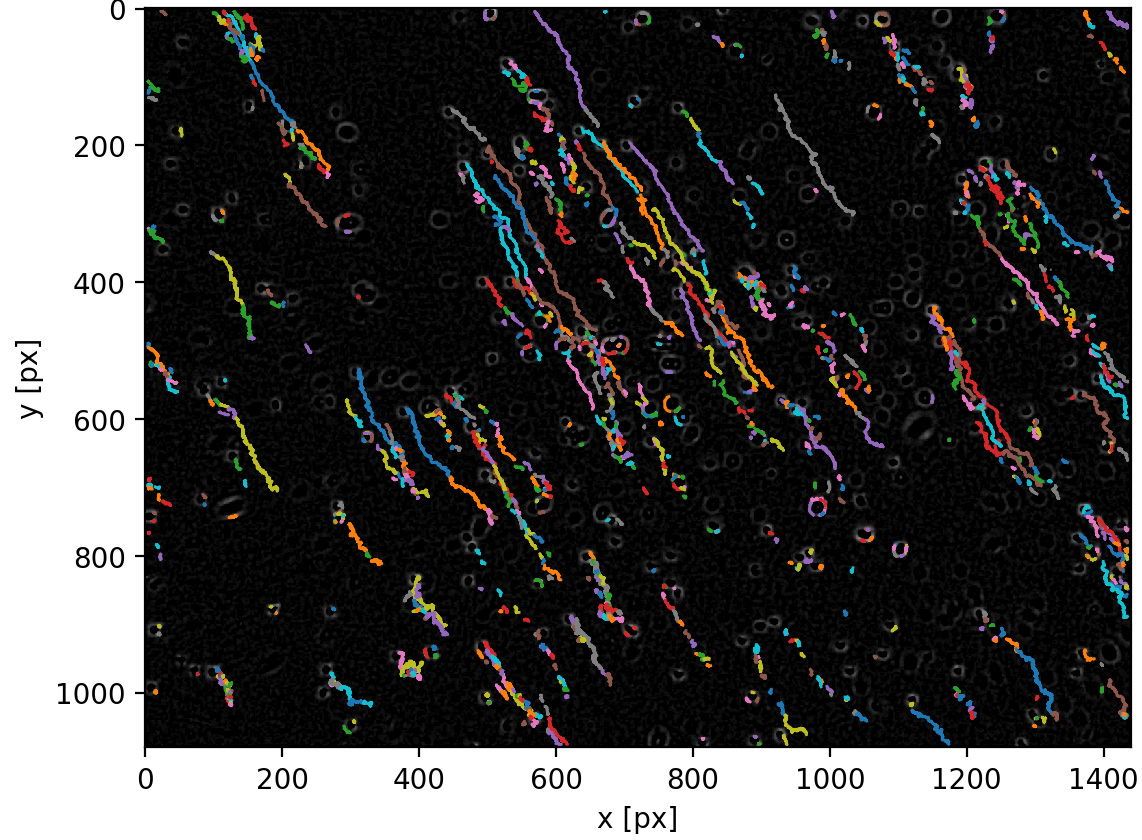
\includegraphics[width=0.48\textwidth]{figures/brownian_trajectories.png}
    \caption{Sample bead trajectories obtained from video microscopy. Although the motion is dominated by thermal fluctuations, the trajectories show a small but consistent drift in one direction. This likely results from slow convection or mechanical stage drift. I subtracted this drift before computing the diffusion statistics.}
    \label{fig:trajectories}
\end{figure}

Although Brownian motion should ideally have no preferred direction, I noticed that many trajectories had a common drift. To focus on the true random part of the motion, I calculated the mean drift velocity of all the beads and subtracted this value from each individual velocity measurement before continuing the analysis.

\subsubsection*{Image Scaling and Velocity Extraction}

To convert pixel displacements into physical distances, I calibrated the image scale using the known diameter of the polystyrene beads. The beads have a nominal diameter of $1~\mu\text{m}$. By examining images of well-focused beads, I measured their apparent diameter to be about 4 pixels. This gives a conversion factor of
\[
    4~\text{pixels} \rightarrow 1~\mu\text{m}.
\]

Since the beads are uniform in size and nearly spherical, and since I only used in-focus images, this calibration offers a reliable estimate of the spatial scale.

Knowing the camera frame rate, I calculated each bead’s instantaneous velocity in $\mu\text{m/s}$ from its frame-to-frame displacement. After taking out the mean drift, I created the distribution of residual velocities and calculated the root-mean-square (RMS) value,
\[
    v_{\mathrm{rms}} = \sqrt{\langle v_x'^2 + v_y'^2 \rangle}.
\]

\subsubsection*{Einstein–Smoluchowski Method for Determining $k_B$}

For short time intervals equal to the video frame spacing $\tau$, the diffusion coefficient $D$ relates to the RMS velocity by
\begin{equation}
    v_{\mathrm{rms}}^2 = \frac{2D}{\tau}.
    \label{eq:v2D}
\end{equation}
This comes from the mean-squared displacement of free Brownian motion,
\[
    \langle \Delta r^2(\tau) \rangle = 4D\tau,
\]
because the measured velocity over one frame interval is $\Delta r / \tau$.

The Einstein–Smoluchowski relation connects the diffusion coefficient to Boltzmann’s constant:
\begin{equation}
    D = \frac{k_B T}{6 \pi \eta r},
    \label{eq:einstein}
\end{equation}
where $r\approx 1\mu\text{m}$ is the bead radius and $\eta\approx 1.0 \text{mPa}\cdot \text{s}$ is the viscosity of water. By combining Eqs.~(\ref{eq:v2D}) and (\ref{eq:einstein}), I derived an expression for $k_B$ based on the measured RMS velocity:
\begin{equation}
    k_B =
    \frac{3\pi\eta r\, v_{\mathrm{rms}}^2\, \tau}{T}.
    \label{eq:kB_from_vrms}
\end{equation}

Using this method, I analyzed three independent videos of bead motion. The resulting values of $k_B$ were:
\[
    k_{B,1} = 1.337\times10^{-23}\,\mathrm{J/K},
\]
\[
    k_{B,2} = 1.353\times10^{-23}\,\mathrm{J/K},
\]
\[
    k_{B,3} = 1.373\times10^{-23}\,\mathrm{J/K}.
\]

\subsubsection*{Final Result and Uncertainty}

I calculated the weighted average of the three measurements. Since all three values are close, I treated them with equal weighting. The mean is
\[
    \bar{k}_B =
    \frac{1.337 + 1.353 + 1.373}{3}\times10^{-23}
    = 1.354\times10^{-23}\,\mathrm{J/K}.
\]

The standard deviation of the three measurements is
\[
    \sigma =
    1.8\times10^{-25}\,\mathrm{J/K},
\]
and the standard error of the mean is
\[
    \Delta\bar{k}_B = \frac{\sigma}{\sqrt{3}}
    = 1.0\times10^{-25}\,\mathrm{J/K}.
\]

Thus, my Brownian-motion-based result is
\[
    k_B = (1.354 \pm 0.010)\times10^{-23}\,\mathrm{J/K}.
\]

This value agrees with the accepted
\[
    k_B^\mathrm{accepted} = 1.380\,649\times10^{-23}\,\mathrm{J/K}
\]
to within a few percent. This demonstrates that video microscopy of micron-scale Brownian motion is a reliable method for determining Boltzmann’s constant.

\section*{Conclusion}

In this experiment, I determined Boltzmann's constant using two independent forms of thermal motion in a colloidal suspension. These were the equilibrium sedimentation profile of micron-scale beads and their Brownian movements in the horizontal plane. The depth-counting method, which fits the exponential decay predicted by the Law of Atmospheres, yielded 

\[
k_B = (1.34 \pm 0.18) \times 10^{-23}\,\mathrm{J/K}.
\]

The analysis of Brownian motion, which used the RMS velocity of tracked particles along with the Einstein-Smoluchowski relation, produced a more accurate result:

\[
k_B = (1.354 \pm 0.010) \times 10^{-23}\,\mathrm{J/K}.
\]

Both measurements align reasonably well with the accepted value of Boltzmann's constant:

\[
k_B^\mathrm{accepted} = 1.380\,649 \times 10^{-23}\,\mathrm{J/K},
\]

as reported by the Encyclopaedia Britannica. \cite{BritannicaBoltzmann} The sedimentation method shows larger uncertainty due to issues with microscope depth calibration, bead detection, and effective-mass estimation. In contrast, the Brownian motion technique benefits from averaging over many particle paths, making it more reliable.

Overall, this investigation shows that we can derive macroscopic thermodynamic constants from microscopic fluctuations. The experiment clearly illustrates the link between random thermal motion, diffusive behavior, and fundamental constants of nature.

\bibliographystyle{apsrev4-2}
\bibliography{report}

\end{document}